\chapter{有机镁试剂}\label{ch:b1:organomagnesium}

多数有用的有机分子的碳原子数，远多于任何廉价的
起始原料，因此合成的核心问题是把两个
碳骨架通过新的 C--C 键连接起来。在碳化合物中，碳
几乎总是化学键中缺电子的一方——与氧成键、与
卤素成键——而两个缺电子的碳彼此不会发生反应。
二十世纪之初，一种由卤代烷与镁在同一烧瓶中制得的
试剂扭转了这一局面：其中的碳富电子，是
亲核试剂，能进攻羰基的碳。借助它，
几乎任何骨架的醇都能由较小的片段构建。本
章将说明该试剂如何制备、为何需要完全干燥的
烧瓶、能与何种物质加成，以及如何规划使用它的合成路线。

\begin{recall}
电负性（\cref{ch:b1:periodicity}）；路易斯酸碱及
配位键（\cref{ch:b1:lewis-resonance-vsepr}）；亲核试剂、
亲电试剂、弯箭头以及有机物种的 $\mathrm{p}K_a$ 标度
（\cref{ch:b1:electronic-effects}）；醇的级数
（伯、仲、叔）与其所连碳原子的级数一致。
\end{recall}

\section{制备格氏试剂}

\begin{definition}[有机金属化合物、格氏试剂]\label{def:b1:organomagnesium:organometallic}
称至少含有一个碳–金属键的化合物为\emph{有机金属化合物}\index{有机金属化合物}。
含 C--Mg 键的化合物称为\emph{有机镁化合物}\index{有机镁化合物}，
其中最常见的一种是
\emph{格氏试剂}\index{格氏试剂} \ce{RMgX}（X = Cl、Br、I），
由卤代烷或卤代芳烃与镁在醚中制得，
反应为 \ce{R-X + Mg -> R-MgX}。
\end{definition}

镁插入 C--X 键中。醚并非惰性溶剂：
\ce{RMgX} 中的镁周围仅有四个价电子，
两个醚分子各以一对孤电子对与镁配位，
使其达到八电子结构，并使试剂保持在溶液中。

\begin{omfigure}
\begin{tikzpicture}[font=\small]
  \node (mg) at (0,0) {Mg};
  \node (r) at (-1.5,0) {R};
  \node (x) at (1.5,0) {Br};
  \node (o1) at (0,1.45) {O};
  \node (o2) at (0,-1.45) {O};
  \draw[thick] (r) -- (mg) -- (x);
  \draw[thick, ->, omDef] (o1) -- (mg);
  \draw[thick, ->, omDef] (o2) -- (mg);
  \draw (o1) -- ++(-0.8,0.45) node[left] {\ce{CH3CH2}};
  \draw (o1) -- ++(0.8,0.45) node[right] {\ce{CH2CH3}};
  \draw (o2) -- ++(-0.8,-0.45) node[left] {\ce{CH3CH2}};
  \draw (o2) -- ++(0.8,-0.45) node[right] {\ce{CH2CH3}};
  \node[align=left, anchor=west] at (3.2,0) {两个醚分子各给出一对孤电子对（蓝色）：\\四面体构型的镁，\\八电子结构};
\end{tikzpicture}

{\small 乙醚（二乙醚）中的格氏试剂。
氧–镁配位键解释了为何该试剂只能在
醚或类似的路易斯碱中生成。}
\end{omfigure}

\begin{method}[制备格氏试剂]\label{met:b1:organomagnesium:prepare}
\begin{enumerate}
  \item 将所有玻璃仪器在烘箱中烘干；冷凝管上接
        氯化钙干燥管，并使用无水乙醚。
  \item 将镁屑和少量乙醚加入三口烧瓶中，
        该烧瓶配有冷凝管、滴液漏斗和搅拌器。
  \item 加入少量卤化物，待反应开始（
        溶液变浑浊、乙醚轻微沸腾）时，将其余卤化物
        逐滴加入，滴加速度应使体系保持缓和回流。
  \item 立即在同一干燥装置中使用该溶液。
\end{enumerate}
\end{method}

\begin{omfigure}
\begin{tikzpicture}[font=\small]
  \pic at (0,-0.05) {stirrer};
  \pic (f) at (0,0.05) {threeneck={0.35}{omDef!14}};
  \pic at (f-c) {condenser};
  \pic at ($(f-c)+(0,3.2)$) {guardtube};
  \pic[rotate=25] at (f-l) {dropfunnel={0.5}{orange!20}};
  \fill[black!45, rotate around={-25:(f-r)}] ($(f-r)+(-0.17,0)$) rectangle ++(0.34,0.3);
  \draw[->] (2.4,0.9) node[right] {干燥乙醚中的镁屑} -- (0.6,0.6);
  \draw[->] (-3.0,3.9) node[left, align=right] {乙醚中的卤化物，\\逐滴加入} -- (-1.8,3.4);
  \draw[->] (1.8,5.3) node[right] {冷凝管（冷却水）} -- (0.45,4.8);
  \draw[->] (1.8,6.6) node[right] {氯化钙干燥管} -- (0.3,6.4);
  \draw[->] (2.4,-0.2) node[right] {磁力搅拌器} -- (1.3,-0.2);
\end{tikzpicture}

{\small 格氏反应装置：凡是空气能够接触的部分，
都必须干燥。空气中的水蒸气被干燥管截留；
冷凝管使沸腾的乙醚回流入烧瓶。}
\end{omfigure}

\begin{inthelab}[必须先引发的反应]
格氏试剂的制备有时无法开始：镁表面覆盖着一层
氧化膜。用玻璃棒压碎一小段镁屑、加入
一小粒碘晶体，或局部加热烧瓶，均可使新鲜金属暴露出来。
反应一旦开始便放热，乙醚会自行沸腾；
此时应减慢滴加速度，以免溢出。乙醚
沸点为 \qty{35}{\celsius}，其蒸气极易燃烧：
实验室内任何地方都不得有明火，并应备好冰浴。
% ledger: bp:diethylether
\end{inthelab}

\section{强碱与亲核试剂}

\begin{definition}[极性反转]\label{def:b1:organomagnesium:umpolung}
镁的电负性（1.31）远低于
碳（2.55）：在 \ce{R-MgX} 中，C--Mg 键被极化，
负端位于碳原子上，该碳起碳负离子的作用。在卤代烷 \ce{R-X} 中，
同一碳原子带正电（Br 的电负性为 2.96）。将亲电碳
变为亲核的碳，称为\emph{极性反转}\index{极性反转}。
% ledger: en:Mg, en:C, en:Br
\end{definition}

\begin{proposition}[格氏试剂会被酸性氢破坏]\label{prop:b1:organomagnesium:base}
格氏试剂可与水、醇、羧酸、
带 N--H 键的胺及端炔定量反应，生成烷烃
\ce{R-H}: \ce{RMgX + H2O -> R-H + Mg(OH)X}.
\end{proposition}

\begin{proof}
类碳负离子的碳是共轭酸碱对 \ce{R-H}/\ce{R^-} 中的碱，
烷烃是有机化学中远为最弱的酸：在水中
无法测得质子从它们上脱离，水中能存在的最强碱为氢氧根
（见\cref{ch:b1:predominant-reaction}，拉平效应）。列表中的任何酸都
强得多，质子转移到 \ce{R^-} 上的
平衡常数极大：反应完全且迅速。
\end{proof}

这就是要求仪器干燥的原因：一滴水会破坏
等量的试剂。变害为利，\ce{CH3CH2MgBr + D2O}
可恰好在溴原来所在的位置上引入一个氘原子。

\section{羰基化合物与二氧化碳的加成}

C=O 基团中的碳是亲电碳
（见\cref{ch:b1:electronic-effects}）。格氏试剂将其 R 基团加到该碳上，
C=O 的 $\pi$ 电子对转到氧上；随后经酸性后处理，
使醇盐质子化。

\begin{omfigure}
\setchemfig{atom sep=2.1em}
\schemestart
\chemfig{@{r}R-[@{rm}]MgBr}
\+
\chemfig{@{cc}C(-[:150]R')(-[:210]R'')=[@{co}]@{o}O}
\arrow{->}
\chemfig{C(-[:150]R')(-[:210]R'')(-[2]R)-O^{-}}
\chemfig{\phantom{.}}\chemfig{^{+}MgBr}
\arrow{->[\ce{H3O+}]}
\chemfig{C(-[:150]R')(-[:210]R'')(-[2]R)-OH}
\schemestop
\chemmove{\draw[->, thick, shorten <=2pt, shorten >=2pt](rm) .. controls +(70:9mm) and +(180:7mm) .. (cc);
          \draw[->, thick, shorten <=2pt, shorten >=2pt](co) .. controls +(90:6mm) and +(90:6mm) .. (o);}
\par\vspace{6pt}

{\small 格氏试剂对酮（或醛，
$\mathrm{R''} = \mathrm{H}$）的加成：C--Mg 键形成新的 C--C 键，同时 C=O 的 $\pi$
电子对转到氧上；醇镁盐被稀酸质子化，
在单独的一步中完成。}
\end{omfigure}

\begin{proposition}[由羰基化合物制备醇]\label{prop:b1:organomagnesium:carbonyl-addition}
经酸性后处理后，格氏试剂 \ce{RMgX} 可得：与甲醛反应，得
伯醇 \ce{RCH2OH}；与其他醛 $\mathrm{R'CHO}$ 反应，得仲醇
$\mathrm{RR'CHOH}$；与酮 $\mathrm{R'COR''}$ 反应，得叔醇
$\mathrm{RR'R''COH}$。新形成的 C--C 键将 R 连到原羰基碳上。
\end{proposition}

\begin{proof}
羰基碳保留原有的两个取代基，并获得 R 和一个 OH
（来自醇盐的氧）：甲醛带入两个 H，醛带入一个 H 和
一个碳基团，酮带入两个碳基团。醇的级数
即该碳上碳基团的数目：一、二或三。
\end{proof}

\begin{proposition}[由二氧化碳制备羧酸]\label{prop:b1:organomagnesium:co2}
将格氏试剂倒在固体二氧化碳（干冰）上，经酸化后
得到比原来多一个碳的羧酸 \ce{RCOOH}：
\ce{RMgX + CO2 -> RCOOMgX}，然后 \ce{RCOOMgX + H3O+ -> RCOOH + Mg^2+ + X- + H2O}。
\end{proposition}

\begin{proof}
\ce{CO2} 是羰基化合物，其碳原子的受攻方式与
酮相同；生成的羧酸根过于不活泼，
在这些条件下不能再加入第二个 R 基团（带负电荷的羰基
是较差的亲电试剂）。酸使其质子化。
\end{proof}

\section{构建碳骨架}

\begin{method}[设计醇的合成路线]\label{met:b1:organomagnesium:plan-alcohol}
\begin{enumerate}
  \item 找出目标醇中连有 OH 的碳原子。
  \item 选取其中一个碳基团作为 R（它将来自
        由 \ce{R-Br} 制备的格氏试剂）；分子的其余部分
        以该碳作 C=O，即为羰基组分。
  \item 列出所有可能的选择（每个碳基团对应一种），并优先选用
        试剂简单易得的方案。
  \item 检查两个反应物中均不含酸性氢，
        也不含会一并反应的第二个羰基。
\end{enumerate}
\end{method}

\begin{example}[2-苯基丁-2-醇]\label{ex:b1:organomagnesium:plan}
连有 OH 的碳原子上连着一个苯基、一个甲基和一个乙基。
有三种方案：溴化苯基镁与丁-2-酮；溴化甲基镁
与 1-苯基丙-1-酮；溴化乙基镁与
1-苯基乙-1-酮（苯乙酮）。三种方案都可行；最后一种用到两种
最常用的试剂。
\end{example}

\begin{history}[维克多·格林尼亚]
\begin{minipage}[t]{0.2\linewidth}\vspace{0pt}
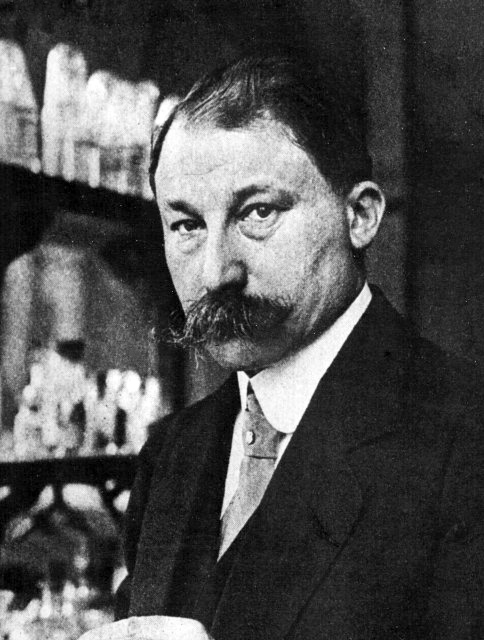
\includegraphics[width=\linewidth]{images/book2/grignard.jpg}
\end{minipage}\hfill
\begin{minipage}[t]{0.76\linewidth}\vspace{0pt}
该试剂以维克多·格林尼亚的名字命名。他作为博士生，
于二十世纪之交发现，镁能溶解在
卤代烷的醚溶液中，且该溶液可加成到
羰基化合物上。其简便性——一种金属、一种溶剂、一只烧瓶——
使其成为本世纪应用最广的碳–碳键形成反应，
并使其发现者获诺贝尔化学奖。
（照片：公有领域，维基共享资源。）
\end{minipage}
\end{history}

\section{练习}

\begin{exercise}[$\star$]\label{exo:b1:organomagnesium:1}
写出溴化乙基镁和溴化苯基镁的制备反应，
给出 C--Br 键和 C--Mg 键的极化情况，
并结合电负性说明。
\end{exercise}

\begin{exercise}[$\star$]\label{exo:b1:organomagnesium:2}
碘化甲基镁与下列物质反应分别生成什么：水；乙醇；乙酸；
重水 \ce{D2O}？写出反应方程式。
\end{exercise}

\begin{exercise}[$\star$]\label{exo:b1:organomagnesium:3}
给出溴化乙基镁与甲醛、乙醛、丙酮、苯甲醛和二氧化碳
反应（经酸性后处理）所得的生成物，
并给出每种醇的级数。
\end{exercise}

\begin{exercise}[$\star$]\label{exo:b1:organomagnesium:4}
为什么不能用 4-溴丁-1-醇制备格氏试剂？
\end{exercise}

\begin{exercise}[$\star\star$]\label{exo:b1:organomagnesium:5}
写出溴化甲基镁与乙醛加成的反应机理，
以及后处理过程，均用弯箭头表示；产物是否具有手性？
产物是否以单一对映异构体的形式得到？为什么？
\end{exercise}

\begin{exercise}[$\star\star$]\label{exo:b1:organomagnesium:6}
试提出两种由格氏试剂
与酮制备 3-甲基戊-3-醇的方法。
\end{exercise}

\begin{exercise}[$\star\star$]\label{exo:b1:organomagnesium:7}
如何由 2-溴丙烷制备 2-甲基丙酸？计算
以 \qty{12.3}{g} 溴代物为原料，在
产率为 \qty{70}{\percent} 时所得酸的质量（$M$：\ce{C3H7Br} \qty{123.0}{g/mol}，\ce{C4H8O2}
\qty{88.0}{g/mol}）。
\end{exercise}

\begin{exercise}[$\star\star$]\label{exo:b1:organomagnesium:8}
一名粗心的学生以 \qty{0.0500}{mol} 溴苯为原料，
在含 \qty{0.18}{g} 水的乙醚中制备溴化苯基镁。
试问有多大比例的试剂被破坏？生成了哪种产物？
\end{exercise}

\begin{exercise}[$\star\star$]\label{exo:b1:organomagnesium:9}
联苯 \ce{C6H5-C6H5} 是制备溴化苯基镁时的副产物。
试提出其生成途径，并说明为何向过量镁中
缓慢加入溴苯可以限制其生成。
\end{exercise}

\begin{exercise}[$\star\star\star$]\label{exo:b1:organomagnesium:10}
试由格氏试剂设计两条合成 1-苯基乙-1-醇的路线，以及
一条合成 2-苯基丙-2-醇的路线。对每条路线，
指出生成该格氏试剂的卤代烷。
\end{exercise}

\begin{exercise}[$\star\star\star$]\label{exo:b1:organomagnesium:11}
解释为什么格氏试剂与羰基化合物必须按
下题所选定的顺序混合，以及后处理为何要
用冷的稀酸而不是单用水。
\end{exercise}

\begin{exercise}[$\star\star\star$]\label{exo:b1:organomagnesium:12}
由 \qty{0.100}{mol} 某溴代物制得的格氏试剂，
取一份试样倒入过量水中，生成的碱式镁盐
用盐酸滴定；折算到整个溶液，
共需 \qty{0.088}{mol} 盐酸。说明其原理，并求该制备的
产率。
\end{exercise}

\section{问题：三苯甲醇}

\begin{problem}[{周末问题——制备溴化苯基镁，
其与二苯甲酮的加成、后处理，以及
三苯甲醇的产率}]
\label{pb:b1:organomagnesium:1}
在干燥的三口烧瓶中，将 \qty{0.535}{g} 镁与
\qty{3.14}{g} 溴苯在无水乙醚中反应，制得溴化苯基镁。
将 \qty{3.28}{g} 二苯甲酮
\ce{(C6H5)2CO} 溶于同种乙醚中所得的溶液，随后逐滴加入。经
冷稀硫酸后处理、萃取及重结晶后，
得到 \qty{3.75}{g} 纯三苯甲醇 \ce{(C6H5)3COH}，
并分离出 \qty{0.15}{g} 联苯。摩尔质量（\unit{g/mol}）：
Mg 24.3, \ce{C6H5Br} 156.9, \ce{C13H10O} 182.0, \ce{C19H16O} 260.0,
\ce{C12H10} 154.0, \ce{C7H6O2} 122.0.

\medskip
\noindent\textbf{第一部分——溴化苯基镁。}
\begin{enumerate}
  \item 写出制备反应的方程式。
  \item 计算镁与溴苯的物质的量，哪一种
        过量？
  \item 为什么装置必须干燥？写出与水的反应。
  \item 干燥管的作用是什么？
  \item 除溶解试剂外，乙醚为何必不可少？
  \item 联苯来自试剂与溴苯的反应。
        写出该反应，并计算因此损失的溴苯的物质的量。
\end{enumerate}

\medskip
\noindent\textbf{第二部分——加成反应。}
\begin{enumerate}[resume]
  \item 计算二苯甲酮的物质的量。
  \item 用弯箭头写出加成反应的机理。
  \item 哪种试剂限制了三苯甲醇的生成？
        请结合第一部分的结果。
  \item 三苯甲醇是否具有手性？请说明理由。
  \item 为什么将二苯甲酮加入试剂中，而不是反过来？
  \item 二苯甲酮溶液中痕量的水会有什么影响？
\end{enumerate}

\medskip
\noindent\textbf{第三部分——后处理。}
\begin{enumerate}[resume]
  \item 写出醇盐的质子化反应。
  \item 为什么使用冷的稀酸，而不是只用水？
  \item 三苯甲醇和镁盐经乙醚萃取后，
        分别位于何处？
  \item 如何将联苯与三苯甲醇分离？（联苯在
        冷的轻石油醚中的溶解度大得多。）
  \item 用何种检验可以确定晶体的纯度？
  \item 三苯甲醇在冷的稀酸中不发生变化，但
        能溶于浓硫酸，生成深黄色的碳正离子。
        写出其生成过程，并解释其稳定性（可与
        \cref{ch:b1:electronic-effects}对照）。
\end{enumerate}

\medskip
\noindent\textbf{第四部分——产率与另一产物。}
\begin{enumerate}[resume]
  \item 计算所得三苯甲醇的物质的量。
  \item 计算相对于限量试剂的产率。
  \item 提出两个造成损失的原因。
  \item 若将第一部分的试剂（已校正联苯的影响）
        改为倒在固体二氧化碳上，则会生成何种产物？
  \item 计算该产物的理论质量。
  \item 写出该羧化反应的方程式。
  \item 以百分数表示三苯甲醇的产率。
\end{enumerate}
\end{problem}
